% !TeX spellcheck = it_IT

\documentclass[format=169, handout]{beamer}

\usepackage[utf8]{inputenc}
\usepackage[italian]{babel}
\usepackage{hyperref}
\usepackage{xcolor}
\usepackage{listings}

% for matlab code
\definecolor{mygreen}{RGB}{28,172,0} % color values Red, Green, Blue
\definecolor{mylilas}{RGB}{170,55,241}
\definecolor{mGray}{rgb}{0.5,0.5,0.5}
\definecolor{mPurple}{rgb}{0.58,0,0.82}
\definecolor{backgroundColour}{rgb}{0.95,0.95,0.92}

\lstdefinestyle{matlab}{language=Matlab,%
	%basicstyle=\color{red},
	breaklines=true,%
	morekeywords={matlab2tikz},
	keywordstyle=\color{blue},%
	morekeywords=[2]{1}, keywordstyle=[2]{\color{black}},
	identifierstyle=\color{black},%
	stringstyle=\color{mylilas},
	commentstyle=\color{mygreen},%
	showstringspaces=false,%without this there will be a symbol in the places where there is a space
	numbers=left,%
	numberstyle={\tiny \color{black}},% size of the numbers
	numbersep=9pt, % this defines how far the numbers are from the text
	emph=[1]{for,end,break},emphstyle=[1]\color{red}, %some words to emphasise
	%emph=[2]{word1,word2}, emphstyle=[2]{style},    
}

\usetheme{metropolis}

\usepackage{mathtools}
\DeclarePairedDelimiter{\ceil}{\lceil}{\rceil}

\title{Esercitazioni di Informatica B}
\subtitle{Array in Matlab}

\author{Stefano Cereda\\
	stefano.cereda@polimi.it
}
\date{20/11/2018}
\institute[PoliMi]{\vspace{0.5cm}\centering Politecnico di Milano \\ \vspace{0.2cm}
	
\includegraphics[width=0.2\textwidth]{../logopolimi}}

\setbeamercovered{invisible}

\definecolor{rosso}{rgb}{1,0,0}
\definecolor{verde}{rgb}{0,1,0}
\definecolor{blu}{rgb}{0,0,1}
\definecolor{giallo}{rgb}{1,1,0}
\definecolor{magenta}{rgb}{1,0,1}
\definecolor{ciano}{rgb}{0,1,1}


\makeindex

\begin{document}

\begin{frame}
	\maketitle
\end{frame}

\begin{frame}{Operazioni su matrici}
Date le seguenti matrici $a$ e $b$ si dica cosa stampano le seguenti istruzioni.

$a$ =
\begin{tabular}{|ccc|}
	\hline
	1&2&3\\
	4&5&6\\
	7&8&9\\
	\hline
\end{tabular}
$b$ =
\begin{tabular}{|ccc|}
	\hline
	9&8&7\\
	6&5&4\\
	3&2&1\\
	\hline
\end{tabular}

\begin{enumerate}
	\item a(3,1)
	\item a(8)
	\item mod(a,b)
	\item {[r c]}=size(mod(a,b))
\end{enumerate}

\end{frame}

\begin{frame}{Immagini - matrice tridimensionale}
Un'immagine può essere descritta tramite una \emph{matrice tridimensionale} in cui i primi due indici indicano un punto del piano ed il terzo indice viene utilizzato per i colori.

\begin{center}
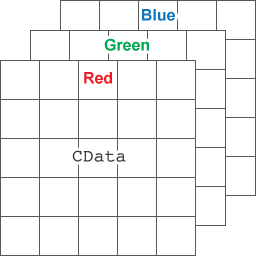
\includegraphics[width=0.2\linewidth]{./matrice_immagine.png}
\end{center}

Il primo indice viene usato per la coordinata $y$ ed il secondo per la coordinata $x$, con l'origine nel punto in alto a sinistra.
Dunque, $M(1,1,:)$ sarà un array monodimensionale che indica il colore del pixel in alto a sinistra.
\end{frame}

\begin{frame}{Immagini - colori}
Il colore di un punto viene descritto da un array di lunghezza 3 in quanto ogni colore può essere descritto come combinazione dei tre colori di base rosso verde e blu.

{
\centering
\begin{tabular}{|c|c|}
	\hline 
	Tripletta RGB & Colore \\ 
	\hline 
	1 0 0 & \textcolor{rosso}{Rosso} \\ 
	0 1 0 & \textcolor{verde}{Verde} \\ 
	0 0 1 & \textcolor{blu}{Blu} \\ 
	1 1 0 & \textcolor{giallo}{Giallo} \\ 
	1 0 1 & \textcolor{magenta}{Magenta} \\
	0 1 1 & \textcolor{ciano}{Ciano} \\ 
	0 0 0 & Nero \\ 
	1 1 1 & Bianco \\ 
	\hline 
\end{tabular}
\par
}


I colori di base vengono anche detti \emph{canali}.
\end{frame}

\begin{frame}[fragile]{Immagini - Bandiera Italiana}
Creiamo un'immagine della bandiera italiana.
Dato che una bandiera ha un rapporto fra le dimensioni di 2:3 creiamo un'immagine con 200 pixel verticali e 300 pixel orizzontali:
\begin{lstlisting}[style=matlab]
bandiera = zeros(200,300,3);
\end{lstlisting}

E dipingiamo le tre bande verticali di verde, bianco e rosso:
\begin{lstlisting}[style=matlab, firstnumber=2]
bandiera(:, 1:100, 2) = 1;
bandiera(:, 101:200, :) = 1;
bandiera(:, 201:300, 1) = 1;
\end{lstlisting}

E mostriamo la figura:
\begin{lstlisting}[style=matlab, firstnumber=5]
imagesc(bandiera);
\end{lstlisting}
\end{frame}

\begin{frame}[fragile, allowframebreaks]{Immagini - Bandiera Italiana - colori float}
Usando triplette RGB con valori 0 o 1 possiamo usare solo 8 colori, se usiamo valori float possiamo indicare molti più colori.

Ad esempio, i colori corretti della bandiera italiana sono:\\
(R:0 G:146 B:70), (R:241 G:242 B:241), (R:206 G:43 B:55)

Le triplette RGB hanno valore massimo 255, dunque possiamo dipingere una bandiera migliore utilizzando dei valori float che indichino questi valori.

Ad esempio, la fascia verde avrà come valore 146/255 per il canale verde e 70/255 per il canale blu.

\url{https://en.wikipedia.org/wiki/RGB_color_model}

\pause

\begin{lstlisting}[style=matlab]
bandiera = zeros(200,300,3);
bandiera(:, 1:100, 2) = 146/255;
bandiera(:, 1:100, 3) = 70/255;

bandiera(:, 101:200, 1) = 241/255;
bandiera(:, 101:200, 2) = 242/255;
bandiera(:, 101:200, 3) = 241/255;

bandiera(:, 201:300, 1) = 206/255;
bandiera(:, 201:300, 2) = 43/255;
bandiera(:, 201:300, 3) = 55/255;
imagesc(bandiera);
\end{lstlisting}

\pause
\centering
\begin{tabular}{cc}
	Colori interi: & 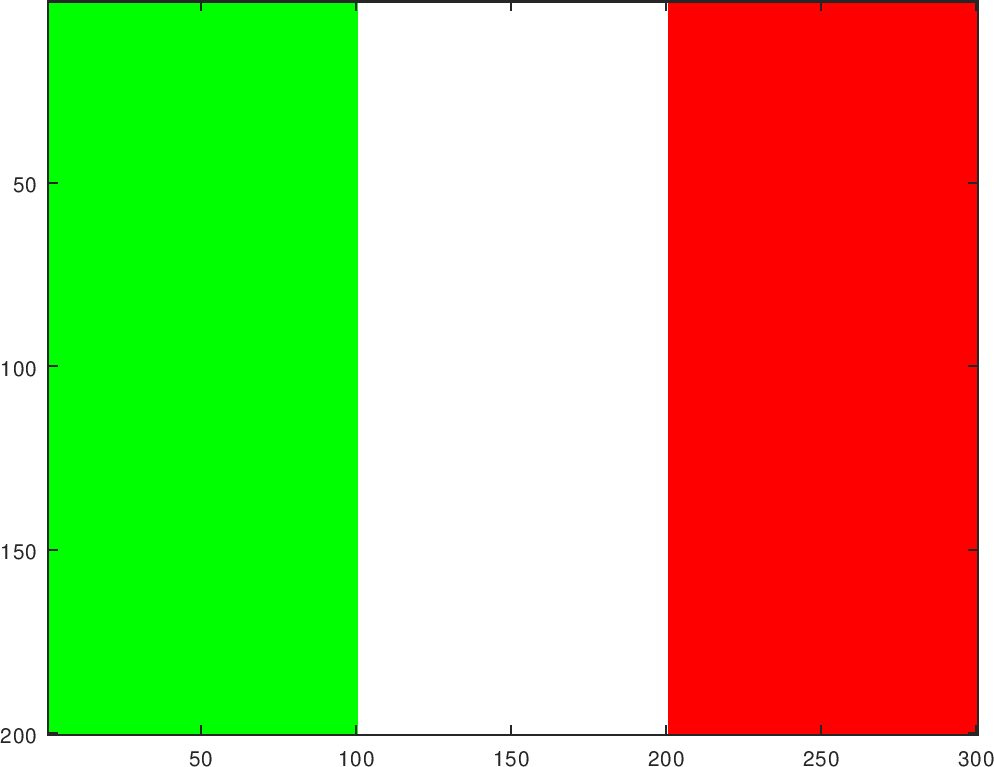
\includegraphics[width=0.4\linewidth]{./bandiera1.png} \\
	Colori float: & 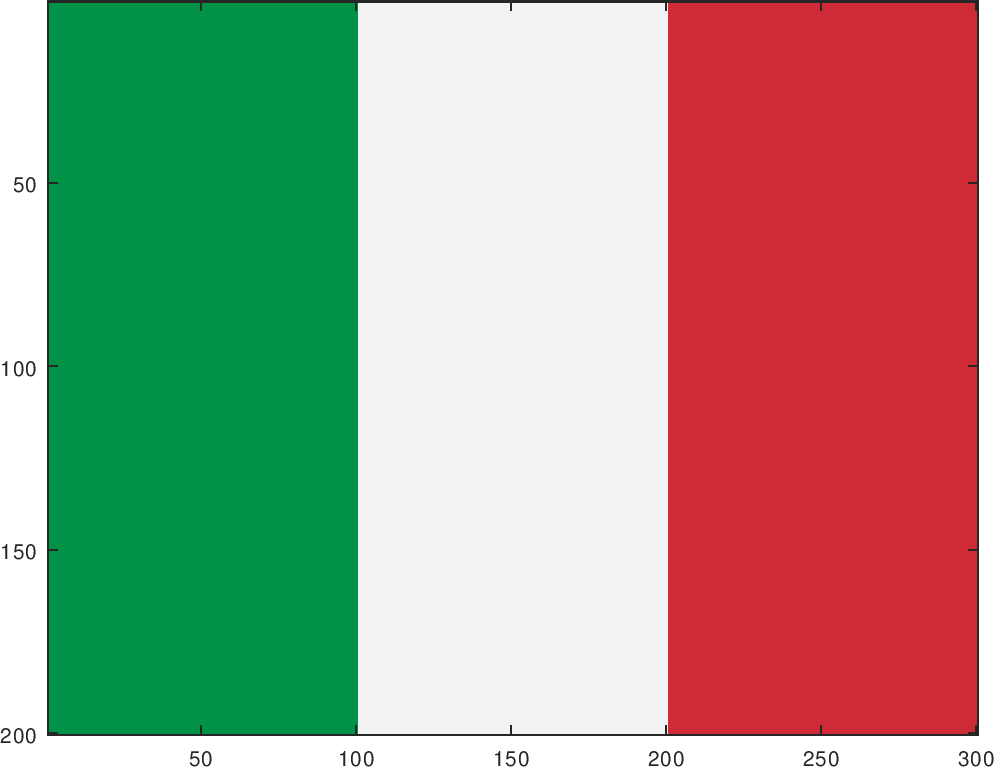
\includegraphics[width=0.4\linewidth]{./bandiera2.png} \\
\end{tabular}
\end{frame}

\begin{frame}[allowframebreaks]{Competizione bandiere}
Quest'anno avete l'opportunità di guadagnare punti extra all'esame con delle competizioni.

La prima competizione riguarda proprio la creazione di una bandiera. Dovrete scrivere del codice matlab che crei l'immagine di una bandiera secondo le seguenti regole:
\begin{enumerate}
	\item Area minima di 200x500 pixel
	\item La bandiera deve essere realizzata interamente con uno script MATLAB, senza interazione con l'utente
	\item È necessario usare operazioni vettoriali, si possono usare cicli
	\item Verrà valutata sia l'estetica della bandiera, sia la struttura del codice utilizzato per realizzarla
	\item Potete presentare una sola bandiera a persona
	\item È necessario caricare nella cartella delle consegne (su beep, corso \emph{Competitions Informatica B}) un file .zip contenente la bandiera (un'immagine .png) e lo script che la genera, opportunamente indentato e commentato. Nel commento in testa al file specificate il vostro nome, cognome, numero di matricola e il vostro docente di Informatica B. È necessario rispettare la scadenza indicata (1/12/2018 ore 23.59).
\end{enumerate}

Verrà assegnato un punto all'esame per il primo classificato/la prima classificata di ogni scaglione.

Iscrivetevi (in beep) al corso \emph{Competitions Informatica B}.

Come disegnare una buona bandiera:
\begin{itemize}
\item \href{https://www.youtube.com/watch?v=BRNzeiV14bY}{The Big Bang Theory - Fun with Flags}
\item \href{https://www.youtube.com/watch?v=pnv5iKB2hl4}{Why city flags may be the worst-designed thing you've never noticed | Roman Mars}
\end{itemize}
\end{frame}

\begin{frame}{Rotazione di matrice}
Sc scriva una script in Matlab/Octave che data una matrice $a$ di dimensioni $N\times N$ crea una nuova matrice $b$ ruotata di 90 gradi in senso antiorario rispetto ad $a$.

Si consideri $N=4$ e la matrice $a$ inizializzata con i valori:

\centering
\begin{tabular}{|cccc|}
	\hline
	1&2&3&4\\
	2&3&4&5\\
	6&7&8&9\\
	0&0&0&0\\
	\hline
\end{tabular}
\end{frame}

\begin{frame}{Sequenza palindroma}
Si scriva uno script che chiede l’inserimento di una sequenza di N numeri e alla fine dice se la sequenza è palindroma o no.

Si ricorda che una sequenza è palindroma se risulta uguale letta da sinistra verso destra o da destra verso sinistra
\end{frame}

\begin{frame}{Confronti}
Si scriva uno script che chiede di inserire una sequenza di N numeri.

Successivamente, si inserisca un ulteriore numero e si dica se tutti i numeri della sequenza sono minori, uguali o maggiori di tale numero.
\end{frame}

\begin{frame}{Confronti con matrici}
Scrivere in Matlab uno script che, data una matrice $m$ di numeri, restituisce in uscita una matrice $mr$, ottenuta da $m$ nel seguente modo:
\begin{itemize}
	\item si calcola la media aritmetica dei valori di $m$;
	\item per i valori che in $m$ sono minori della media, in $m$r si
pone nella stessa posizione il valore -1, per quelli superiori alla media si pone il valore 1, e per gli altri (quelli uguali alla media) si pone lo stesso valore.
\end{itemize}

Si utilizzi la seguente matrice $m$

\centering
\begin{tabular}{|ccc|}
	\hline
	-2&2&3\\
	4&5&6\\
	\hline
\end{tabular}
\end{frame}

\begin{frame}{Inserimento ordinato nell'array}
Scrivere un programma che acquisisce da tastiera una serie di interi e li memorizza in modo ordinato nell'array.

\pause
Se, per esempio, $a = \{1, 3, 4, …\}$ e si vuole inserire 2, i valori 3 e 4 devono essere spostati a destra per fare spazio al nuovo elemento:

\centering
\begin{tabular}{|c|c|c|c|}
	\hline
	1&3&4&...\\
	\hline
\end{tabular}
$\rightarrow$
\begin{tabular}{|c|c|c|c|c|}
	\hline
	1& \alert{2} &3&4&...\\
	\hline
\end{tabular}
\end{frame}

\begin{frame}
\Huge
Esercizi svolti 27/11/2018
\end{frame}

\begin{frame}{Aggiunta colonna}
Scrivere uno script Matlab che, data una matrice $Q$ ed un valore $v$, stampi una
matrice corrispondente a $Q$, alla quale è stata aggiunta una nuova prima
colonna contenente $v$.
\end{frame}

\begin{frame}{Ordinamento matrice}
Ordinare una matrice per righe o per colonne, in ordine crescente o decrescente mantenendo la struttura della matrice. Vedere l'help della funzione sort.

Si crei poi un vettore ordinato contenente tutti gli elementi della matrice.

Infine, si trasformi il vettore in una matrice con le stesse dimensioni della matrice originale. Si veda l'help della funzione reshape.
\end{frame}

\begin{frame}{Vettori logici}
Risolvere i due esercizi di confronto utilizzando vettori logici.
\end{frame}

\begin{frame}{Coppie per somme}
Scrivere uno script MATLAB che, ricevuto in ingresso un intero positivo $n$, stampi due vettori $x$ e $y$, contenenti tutte le coppie di interi $(x,y)$ la cui somma è pari ad $n$.
\end{frame}

\begin{frame}{Soglia intorno}
Si scriva in linguaggio MATLAB uno script che riceva in ingresso una matrice, un numero di riga, un numero di colonna e un valore di soglia. Lo script stampa true se tutti i valori delle celle della matrice nell'intorno della cella della riga e della colonna date sono minori del valore di soglia.

Le celle nell'intorno della cella identificata dalla riga e dalla colonna date sono quelle immediatamente adiacenti a questa cella.
\end{frame}

\begin{frame}{Caffè}
In un dipartimento ci sono 9 persone, ognuna nell'ultima settimana ha
consumato un certo numero di caffè memorizzati in una matrice "caffe" data
(dove le righe rappresentano le persone, mentre le colonne i giorni).
\begin{enumerate}
	\item Si vuole sapere quanto deve pagare ogni persona sapendo che ogni caffè
	ha un costo di 0,25 euro.
	\item Si supponga che vi sia un costo fisso di noleggio della macchinetta per
	fare il caffè pari a 10 euro a settimana.
	\begin{enumerate}
		\item  La metà di tale costo è divisa equamente tra i bevitori (coloro che
		hanno consumato almeno un caffè);
		\item l'altra metà tra i bevitori che ne hanno consumato di più rispetto
		alla media.
	\end{enumerate}
\end{enumerate}

Si dica quanto deve pagare ogni persona.
\end{frame}

\begin{frame}{Matrice palindroma - TdE 2 Luglio 2018}
Data una matrice $N \times M$, essa si definisce palindroma per riga se la riga 1 è uguale alla riga $N$, la riga 2 è uguale alla riga $N-­$1 e così via.
  
Si scriva uno script MATLAB che, data in ingresso una matrice, stampi 1 se la matrice è palindroma per riga o 0 nel caso non lo sia.

Attenzione alla correzione del tema d'esame, contiene un errore!
\end{frame}

\begin{frame}{Matrice dominante - TdE 20 Luglio 2018}
Una matrice quadrata è definita diagonalmente dominante se il valore assoluto di ciascun elemento sulla  
diagonale principale è maggiore della somma dei valori assoluti degli altri elementi sulla stessa riga.

Per esempio, la seguente matrice è diagonalmente dominante:
\begin{tabular}{ccccc}	 
	20 & 2 & 3 & 4 & 5 \\ 	 
	3 & -25 & 5 & 6 & 7 \\ 
	2 & 3 & 23 & 5 & 6 \\  
	8 & 7 & 6 & -30 & 4 \\ 
	2 & 3 & 4 & 5 & 20 \\  
\end{tabular} 

Si scriva uno script MATLAB che, ricevuta una matrice $m$, stampi -1 se $m$ non è quadrata, 0 se quadrata ma non diagonalmente dominante, 1 se quadrata e diagonalmente dominante.
\end{frame}

\end{document}